\section{Theorie}

%Was ist Beugung(Einzelspalt, Gitter, Aperturfunktion, Sinusgitter, Fouriertrafo)
%Laser (nur Eigenschaften)

\subsection{Beugung}

\subsubsection{Allgemeine Definition}

Als Beugung bezeichnet man das Ph\"anomen, dass Licht, welches durch begrenzende \"Offnungen oder an begrenzenden Kanten vorbeil\"auft, von seiner urspr\"unglichen Richtung abgelenkt wird. Hinter dem Hindernis \"uberlagern sich die Teilwellen gem\"a\ss dem Huygenschen Prinzip, welches besagt, dass jeder Punkt einer Wellenfront eine neue Welle induziert. Diese \"uberlagern sich dann und die daraus resultierenden Interferenzerscheinungen werden als Beugung bezeichnet.

\subsubsection{Das Kirchhoff'sche Beugungsintegral}

%Fraunhofer und Fresnelbeugung
%Fouriertransformation

\subsubsection{Anwendungen}

\begin{enumerate}


\item Beugung am Einzelspalt
$$g(x) = \begin{cases} 
	1 & \text{, falls} -\frac{b}{2}<x<\frac{b}{2}\\
	0 & \text{, sonst}
     \end{cases} $$
Man erh\"alt durch Ausrechnen des Beugungsintegrals folgende Abh\"angigkeit f\"ur die Intensit\"at:
$$ I \sim \left(\frac{\sin(\beta)}{\beta}\right)^2 $$
\begin{wrapfigure}{rh}{0.4\textwidth}
	\begin{center}
		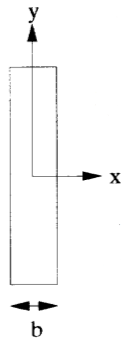
\includegraphics[width=0.1\textwidth]{Bilder/Einzelspalt.jpg}
	\end{center}
	\caption{Einzelspalt}
\end{wrapfigure}
Die Aperturfunktion am Einzelspalt (unter Vernachl\"assigung der Begrenzung in y-Richtung) lautet


Hier ist $\beta = \frac{k}{2b}\sin(\theta)$ und $\theta$ der Einfallswinkel auf dem Schirm vom Ursprung des Spaltes aus.


\item Beugung am Gitter





\end{enumerate}